
\section*{Problema P6.41}

\renewcommand*\thesection{6.41}
\numberwithin{equation}{section}

\begin{center}
    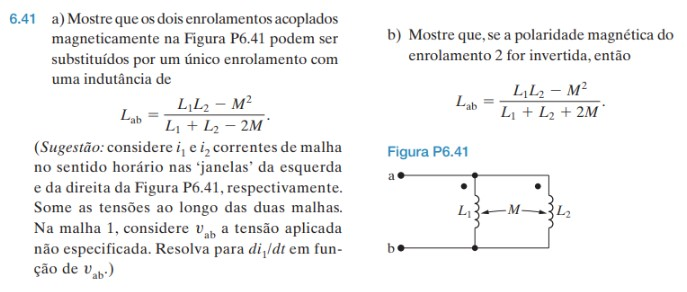
\includegraphics[scale=1.0]{P6.41.jpg}
\end{center}

\subsection*{(a)}

Aplicando análise de malhas no circuito, temos na malha 1:

\[ -v_{ab} + L_1\diff{(i_1 - i_2)}{t} + M\diff{i_2}{t} \]   

\begin{equation}\label{eq:6.41.1}
    v_{ab} = \diff{i_1}{t}\left(L_1\right) + \diff{i_2}{t}\left(M - L_1\right)
\end{equation}

Na malha 2,

\[ L_1\diff{(i_2 - i_1)}{t} - M\diff{i_2}{t} + M\diff{(i_1 - i_2)}{t} + L_2\diff{i_2}{t} = 0 \]   

\begin{equation}\label{eq:6.41.2}
    \diff{i_1}{t}\left(-L_1 + M\right) + \diff{i_2}{t}\left(L_1 - 2M + L_2\right) = 0
\end{equation}

A partir de \eqref{eq:6.41.1} e \eqref{eq:6.41.2} temos o sistema linear

\begingroup
\renewcommand*{\arraystretch}{2}

\[
    \begin{bmatrix}
        L_1 & M - L_1    \\
        M - L_1    & L_1 - 2M + L_2
    \end{bmatrix}
    \begin{bmatrix}
        \diff{i_1}{t} \\
        \diff{i_2}{t}
    \end{bmatrix}
    =
    \begin{bmatrix}
        v_{ab} \\
        0
    \end{bmatrix}
\]

\endgroup

Vamos resolver o sistema aplicando o método de Cramer. Temos

\begingroup
\renewcommand*{\arraystretch}{1.5}

\[ 
    \Delta
    =
    \begin{vmatrix}
        L_1 & M - L_1    \\
        M - L_1    & L_1 - 2M + L_2
    \end{vmatrix}
    =
    L_1^2 - 2ML_1 + L_1L_2 - (M^2 - 2ML_1 + L_1^2)
    =
    L_1L_2 - M^2
\]

\[ 
    \Delta_1
    =
    \begin{vmatrix}
        v_{ab} & M - L_1    \\
        0    & L_1 - 2M + L_2
    \end{vmatrix}
    =
    (v_{ab})(L_1 - 2M + L_2) \quad , \quad
    \Delta_2
    =
    \begin{vmatrix}
        L_1 & v_{ab}   \\
        M - L_1    & 0
    \end{vmatrix}
    =
    (v_{ab})(L_1 - M)
\]

\endgroup

Assim, 

\[ \diff{i_1}{t} = \frac{\Delta_1}{\Delta} = v_{ab}\frac{L_1 - 2M + L_2}{L_1L_2 - M^2} \]

\[ v_{ab} =  \left(\frac{L_1L_2 - M^2}{L_1 - 2M + L_2}\right)\diff{i_1}{t} \]

Usando o fato de que, em um indutor, a tensão é dada por 

\[ v(t) = L\diff{i}{t} \]

Temos que a impedância equivalente ao circuito acima, do ponto de vista dos terminais $a$ e $b$, é

\[ \boxed{L_{eq} = \frac{L_1L_2 - M^2}{L_1 - 2M + L_2}}  \]

\subsection*{(b)}

Invertendo a polaridade magnética de $L_2$, temos que \eqref{eq:6.41.1} e \eqref{eq:6.41.2} se tornam

\[ v_{ab} = \diff{i_1}{t}\left(L_1\right) + \diff{i_2}{t}\left(- M - L_1\right) \]

\[ \diff{i_1}{t}\left(-L_1 - M\right) + \diff{i_2}{t}\left(L_1 + 2M + L_2\right) = 0 \]

Assim, o sistema linear fica como

\begingroup
\renewcommand*{\arraystretch}{2}

\[
    \begin{bmatrix}
        L_1 & - M - L_1    \\
        - M - L_1    & L_1 + 2M + L_2
    \end{bmatrix}
    \begin{bmatrix}
        \diff{i_1}{t} \\
        \diff{i_2}{t}
    \end{bmatrix}
    =
    \begin{bmatrix}
        v_{ab} \\
        0
    \end{bmatrix}
\]

\endgroup

Novamente usando Cramer,

\begingroup
\renewcommand*{\arraystretch}{1.5}

\[ 
    \Delta
    =
    \begin{vmatrix}
        L_1 & - M - L_1    \\
        - M - L_1    & L_1 + 2M + L_2
    \end{vmatrix}
    =
    L_1^2 + 2ML_1 + L_1L_2 - (M^2 + 2ML_1 + L_1^2)
    =
    L_1L_2 - M^2
\]

\[ 
    \Delta_1
    =
    \begin{vmatrix}
        v_{ab} & - M - L_1    \\
        0    & L_1 + 2M + L_2
    \end{vmatrix}
    =
    (v_{ab})(L_1 + 2M + L_2) \quad , \quad
    \Delta_2
    =
    \begin{vmatrix}
        L_1 & v_{ab}   \\
        - M - L_1    & 0
    \end{vmatrix}
    =
    (v_{ab})(L_1 + M)
\]

\endgroup

Assim, 

\[ \diff{i_1}{t} = \frac{\Delta_1}{\Delta} = v_{ab}\frac{L_1 + 2M + L_2}{L_1L_2 - M^2} \]

Com o mesmo raciocínio usado no item (a),

\[ v_{ab} =  \left(\frac{L_1L_2 - M^2}{L_1 + 2M + L_2}\right)\diff{i_1}{t} \]

\[ \boxed{L_{eq} = \frac{L_1L_2 - M^2}{L_1 + 2M + L_2}}  \]



